\startchapter{The Dark Higgs Model}
\label{chapter:dh_model}

The dark matter (DM) search presented in this thesis is motivated by and interpreted with the ``Dark Higgs" (DH) model \cite{Duerr2017}. The DH model predicts a mechanism for DM production from proton-proton collisions at the LHC by means of portal interactions with the dark sector. The dark sector, which is predicted as part of various BSM physics models, represents a collection of quantum fields and associated particles which are assumed to interact gravitationally, but which do not couple via any of the other known forces - electromagnetic, strong and weak - of the SM. Non-gravitational couplings between the dark sector and the SM proceed instead via one or more so-called ``portal mediators". 

In the DH model, the DM is a particle which belongs to the dark sector, and is produced from high-energy \(q\bar{q}\) collisions at the LHC via a hypothetical spin 1 vector boson portal mediator referred to as the \Zprime. The model introduces an additional Higgs boson in the dark sector called the ``Dark Higgs" (DH), which acts as a portal mediator by decaying to SM particles via a small mixing with the SM Higgs boson. 

Figure \ref{fig:Feynman_DH} shows three Feynman diagrams \textcolor{red}{(Note to Bob/self: may need to briefly introduce Feynman diagrams in ch. 1)} which illustrate some of the dominant modes by which the DH model could produce a measurable signature of DM production at the LHC. In all cases, the DM pair is produced via the \Zprime mediator, along with the emission of a DH boson \(s\), which decays to a pair of SM particles. 

\begin{figure}[hp]
	\centering
	\begin{subfigure}[t]{0.49\textwidth}
	\centering
	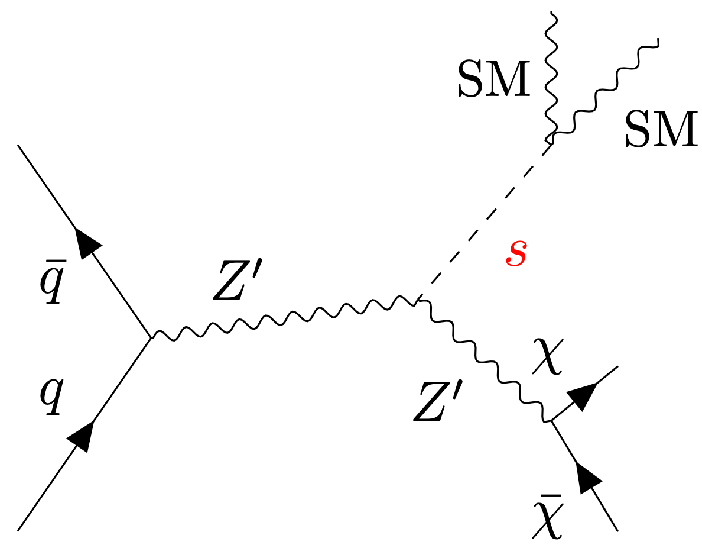
\includegraphics[width=0.95\textwidth]{Figures/2/Fey1.pdf}
%		\begin{tikzpicture}
%			\begin{feynman}
%
%		 		\vertex (a1);
%		 		\vertex[below=7em of a1] (b1);
%		 		\vertex at ($(a1)!0.5!(b1) + (1cm, 0)$) (c1); %z'
%		 		\vertex at ($(a1)!0.4!(b1) + (3cm, 0)$) (c2); %z'
%
%		 		\vertex[right=4cm of a1] (a2); % s
%		 		\vertex[below=5em of a2] (b2); % z'
%
%		 		\vertex at ($(c2) + (1.5cm, 0) + (0,-0.5cm)$) (a3);
%		 		\vertex[below=3em of a3] (b3);
%
%		 		\vertex at ($(a2) + (0, 1cm)$) (a4) ;
%		 		\vertex at ($(a2) + (0, 0.8cm) + (0.8cm, 0)$) (b4) ;
%
%		 		\diagram* {
%		 		  {[edges=fermion]
%		 		    (b1) -- [edge label=\(q\)]( c1) -- [edge label=\(\bar{q}\)](a1),
%		 		    (b3) -- [edge label=\(\bar{\chi}\)] (b2) -- [edge label=\(\chi\)]  (a3),
%		 		  },
%		 		  (c1) -- [boson, edge label=\(Z'\)] (c2),
%		 		  (a2) -- [scalar,edge label=\(\color{red} s\)] (c2) -- [boson, edge label'=\(Z'\)] (b2),
%		 		  (a4) -- [boson, edge label'={\small SM}] (a2) -- [boson, edge label'=\small{SM}] (b4),
%
%		 		};
%		 	\end{feynman}
%		 \end{tikzpicture}
	\caption{s-channel (DH and DM emitted from the \Zprime)}
	\end{subfigure}
		\begin{subfigure}[t]{0.45\textwidth}
	\centering
	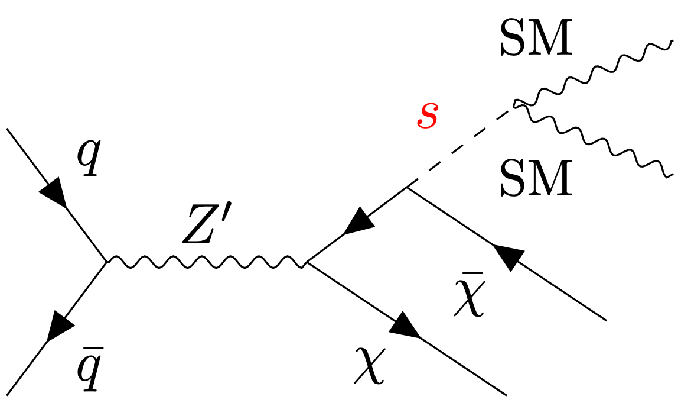
\includegraphics[width=0.95\textwidth]{Figures/2/Fey2.pdf}
%		\begin{tikzpicture}
%			\begin{feynman}
%
%		 		\vertex (b1);
%		 		\vertex at ($(b1) + (-0.75cm, 1cm)$) (a1); %q
%		 		\vertex at ($(b1) + (-0.75cm, -1cm)$) (a2); %qbar
%				\vertex at ($(b1) + (1.5cm, 0cm)$) (c1); %Z'
%				\vertex at ($(c1) + (1.5cm, -1cm)$) (d1); %chi
%				\vertex at ($(c1) + (0.75cm, 0.56cm)$) (d2); %chi
%				\vertex at ($(d2) + (1.5cm, -1cm)$) (d3); %chibar
%				\vertex at ($(d2) + (0.8cm, 0.6cm)$) (e1); %s
%				\vertex at ($(e1) + (1.2cm, 0.5cm)$) (f1); %W
%				\vertex at ($(e1) + (1.2cm, -0.5cm)$) (f2); %W
%				
%				\diagram* {
%				 (a1) -- [fermion, edge label=\(q\)](b1) -- [fermion, edge label=\(\bar{q}\)](a2),
%				 (b1) -- [boson, edge label=\(Z'\)] (c1),
%				 (d3) -- [fermion, edge label=\(\bar{\chi}\)](d2) -- [fermion](c1) -- [fermion, edge label'=\(\chi\)](d1),
%				 (d2) -- [scalar, edge label=\(\color{red} s\)] (e1),
%				 (f1) -- [boson, edge label'={\small SM}](e1) -- [boson, edge label'={\small SM}](f2),
%		 		};
%		 	\end{feynman}
%		 \end{tikzpicture}
	\caption{s-channel (DM emitted from the \Zprime, DH emitted from the DM)}
	\end{subfigure}
	\begin{subfigure}[t]{.42\textwidth}
	\centering
	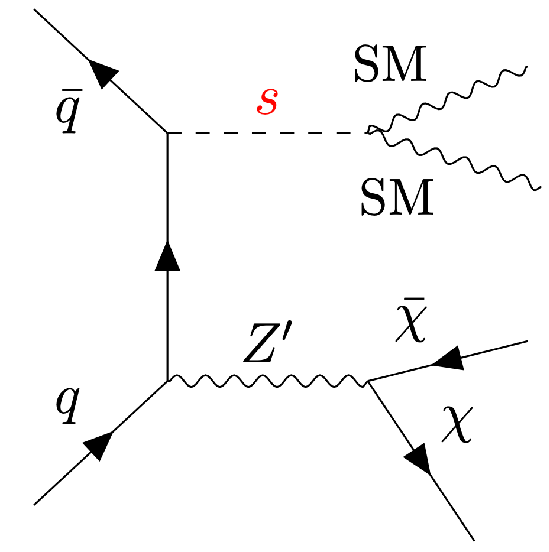
\includegraphics[width=0.95\textwidth]{Figures/2/Fey3.pdf}
%		 \begin{tikzpicture}
%		 	\begin{feynman}
%		 		\vertex (a1); %qbar
%		 		\vertex[below=9em of a1] (b1); %q
%				\vertex at ($(a1)!0.25!(b1) + (1cm, 0)$) (b5); %s
%		 		\vertex at ($(a1)!0.75!(b1) + (1cm, 0)$) (c1); %z'
%		 		\vertex at ($(c1) + (1.5cm, 0) + (0,0)$) (c2); %z'
%
%	         		\vertex[right=1.5cm of b5] (a2); % s
%		 		\vertex[below=2em of a2] (b2); % z'
%
%		 		\vertex at ($(c2) + (0.8cm, 0) + (0,-1.2cm)$) (a3);
%		 		\vertex at ($(c2) + (1.2cm, 0) + (0,0.3cm)$) (b3);
%
%		 		\vertex at ($(a2) + (1.2, 0.5cm)$) (a4) ;
%		 		\vertex at ($(a2) + (0, -0.4cm) + (1.3cm, 0)$) (b4) ;
%
%		 		\diagram* {
%		 		  {[edges=fermion, very thick]
%		 		    (b1) -- [edge label=\(q\)]( c1) -- (b5) -- [edge label=\(\bar{q}\)](a1),
%		 		    (b3) -- [edge label'=\(\bar{\chi}\)] (c2),
%		 		    (c2) -- [edge label=\(\chi\)]  (a3),
%		 		  },
%		 		  {[very thick]
%		 		  (c1) -- [boson, edge label=\(Z'\)] (c2),
%		 		  (b5) -- [scalar,edge label=\(\color{red} s\)] (a2),
%		 		  (a4) -- [boson, edge label'={\small SM}] (a2) -- [boson, edge label'={\small SM}] (b4),
%	         		  }
%		 		};
%		 	\end{feynman}
%		 \end{tikzpicture}
	\caption{t-channel (DH radiated off \(q\), DM emitted from the \Zprime)}
	\end{subfigure}
	\caption{The most contributing Feynman diagrams for DM production at the LHC by means of the DH model}
	\label{fig:Feynman_DH}
\end{figure}


\section{Theoretical Motivation for the Dark Higgs Model}

Given that the particles of the SM acquire mass via their interaction with the Higgs field \cite{HiggsTheory1,HiggsTheory2,HiggsTheory3}, the hypothetical ``Dark Higgs" field - and its associated particle the DH boson - is motivated by the need to likewise generate masses of particles in the dark sector. More generally, the existence of so-called portal mediators which enable interactions between dark sector and SM particles is motivated by theoretical arguments, discussed in Chapter \ref{chapter:introduction} \textcolor{red}{(Note to Bob/self: will point to specific section presenting the thermal freeze-out hypothesis once it's written)}, for the presence of thermal equilibrium between DM and SM particles in the early Universe \cite{DM_earlyUniverse}, which would be established by creation and annihilation processes between the two sectors. The present-day relic abundance of DM, set at the time of thermal freeze-out, places constraints on the details of these creation and annihilation processes. The hypothesized DH boson would open up a new mechanism for portal interactions between DM and SM particles. As discussed in the following section, this new mechanism allows for a relaxation of constraints from the DM relic abundance compared with simpler models in which portal interactions are limited to those mediated by a vector boson mediator (the so-called \Zprime). 

\subsection{Constraints on Generic \Zprime Mediator Models} 

In addition to providing a mechanism by which particles acquire mass in the dark sector, the introduction of a new Higgs boson in the dark sector is motivated by strong theoretical and experimental constraints \cite{Zprime_portal_gen, Zprime_portal_LHC} on the more generic simplified model in which portal interactions between the dark sector and the DM are mediated exclusively by a  vector boson mediator - the so-called \Zprime. Removing the emission of the DH \(s\) from the contributing Feynman diagrams of the DH model in Figure \ref{fig:Feynman_DH} reduces all three to the generic ``s-channel" signature for DM production at the LHC via the \Zprime mediator, shown in Figure \ref{fig:Feynman_Zprime_DM}. 

\begin{figure}[hp]
	\centering
\begin{subfigure}[t]{0.32\textwidth}
	\centering
	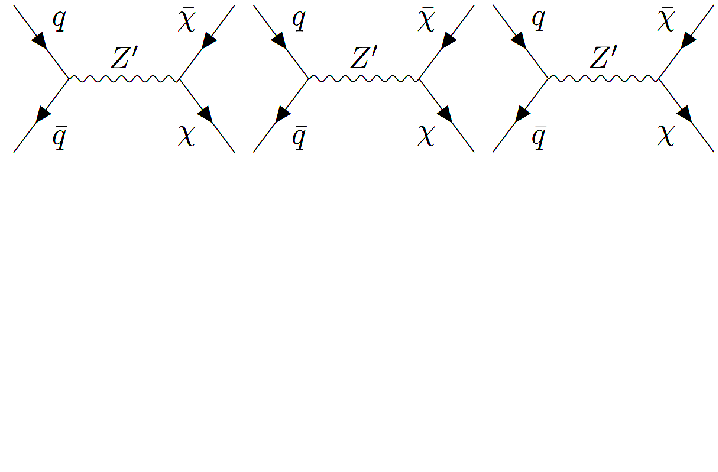
\includegraphics[width=0.8\textwidth]{Figures/2/FeyZprime.pdf}
%		\begin{tikzpicture}
%			\begin{feynman}
%
%		 		\vertex (b1);
%		 		\vertex at ($(b1) + (-0.75cm, 1cm)$) (a1); %q
%		 		\vertex at ($(b1) + (-0.75cm, -1cm)$) (a2); %qbar
%				\vertex at ($(b1) + (1.5cm, 0cm)$) (c1); %Z'
%				\vertex at ($(c1) + (0.75cm, -1cm)$) (d1); %chi
%				\vertex at ($(c1) + (0.75cm, 1cm)$) (d2); %chi
%				
%				\diagram* {
%				 (a1) -- [fermion, edge label=\(q\)](b1) -- [fermion, edge label=\(\bar{q}\)](a2),
%				 (b1) -- [boson, edge label=\(Z'\)] (c1),
%				 (d2) -- [fermion, edge label'=\(\bar{\chi}\)](c1) -- [fermion, edge label'=\(\chi\)](d1);
%		 		};
%		 	\end{feynman}
%		 \end{tikzpicture}
\caption{Generic DM production}
\label{fig:Feynman_Zprime_DM}
\end{subfigure}
\begin{subfigure}[t]{0.32\textwidth}
	\centering
	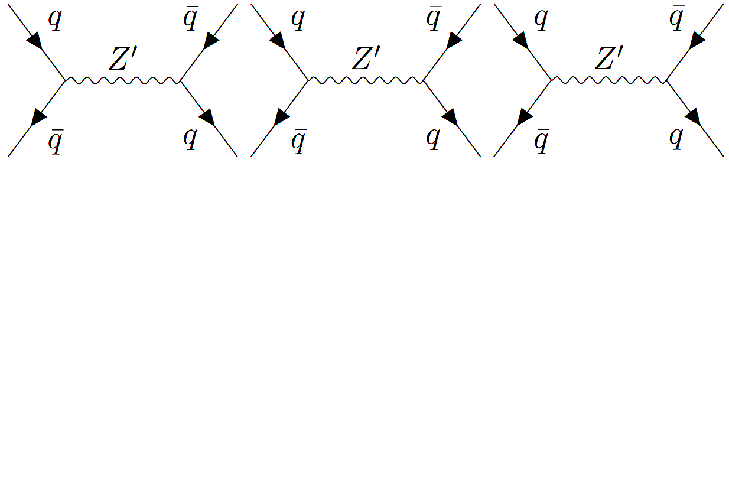
\includegraphics[width=0.8\textwidth]{Figures/2/FeyZprime_dijet.pdf}
%		\begin{tikzpicture}
%			\begin{feynman}
%
%		 		\vertex (b1);
%		 		\vertex at ($(b1) + (-0.75cm, 1cm)$) (a1); %q
%		 		\vertex at ($(b1) + (-0.75cm, -1cm)$) (a2); %qbar
%				\vertex at ($(b1) + (1.5cm, 0cm)$) (c1); %Z'
%				\vertex at ($(c1) + (0.75cm, -1cm)$) (d1); %chi
%				\vertex at ($(c1) + (0.75cm, 1cm)$) (d2); %chi
%				
%				\diagram* {
%				 (a1) -- [fermion, edge label=\(q\)](b1) -- [fermion, edge label=\(\bar{q}\)](a2),
%				 (b1) -- [boson, edge label=\(Z'\)] (c1),
%				 (d2) -- [fermion, edge label'=\(\bar{q}\)](c1) -- [fermion, edge label'=\(q\)](d1);
%		 		};
%		 	\end{feynman}
%		 \end{tikzpicture}
\caption{Dijet resonance}
\label{fig:Feynman_Zprime_dijet}
\end{subfigure}
\begin{subfigure}[t]{0.32\textwidth}
	\centering
	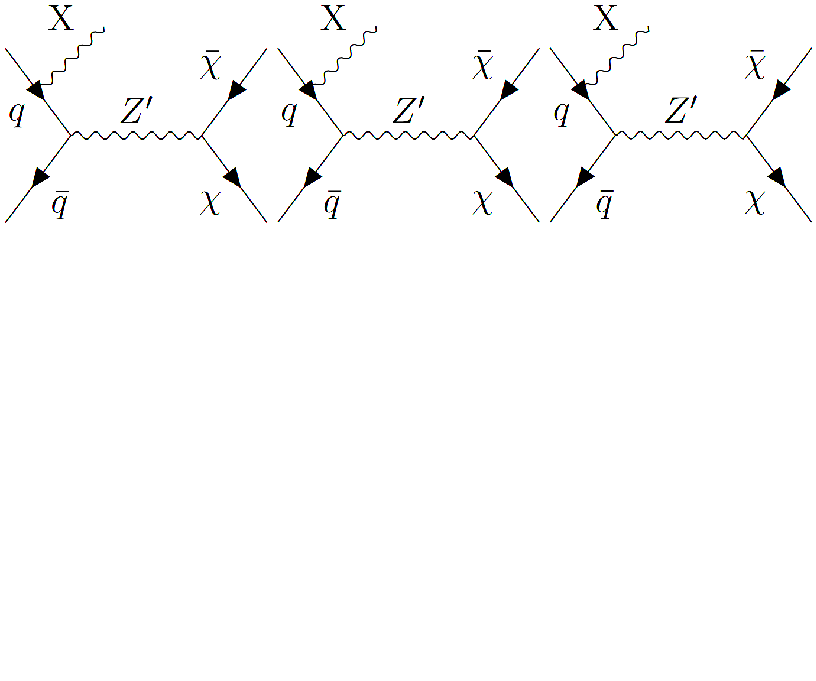
\includegraphics[width=0.8\textwidth]{Figures/2/FeyZprime_monoX.pdf}
%		\begin{tikzpicture}
%			\begin{feynman}
%
%		 		\vertex (b1);
%		 		\vertex at ($(b1) + (-0.75cm, 1cm)$) (a1); %q
%				\vertex at ($(b1) + (-0.375, 0.5cm)$) (s1); %SM
%				\vertex at ($(s1) + (0.75, 0.75cm)$) (s2); %SM
%		 		\vertex at ($(b1) + (-0.75cm, -1cm)$) (a2); %qbar
%				\vertex at ($(b1) + (1.5cm, 0cm)$) (c1); %Z'
%				\vertex at ($(c1) + (0.75cm, -1cm)$) (d1); %chi
%				\vertex at ($(c1) + (0.75cm, 1cm)$) (d2); %chi
%				
%				\diagram* {
%				 (a1) -- [fermion, edge label'=\(q\)](b1) -- [fermion, edge label=\(\bar{q}\)](a2),
%				 (s1) -- [boson, edge label=X,near end](s2),
%				 (b1) -- [boson, edge label=\(Z'\)] (c1),
%				 (d2) -- [fermion, edge label'=\(\bar{\chi}\)](c1) -- [fermion, edge label'=\(\chi\)](d1);
%		 		};
%		 	\end{feynman}
%		 \end{tikzpicture}
\caption{Mono-X signature}
\label{fig:Feynman_Zprime_monoX}
\end{subfigure}
	\caption{Signatures for DM production and detection via a Z' vector boson mediator at the LHC}
	\label{fig:Feynman_Zprime}
\end{figure}

The Z' mediator model is probed at the LHC using either dijet resonance searches \cite{Zprime_portal_gen} in which the \Zprime decays back into a pair of quarks as shown in Figure \ref{fig:Feynman_Zprime_dijet}, or with so-called ``mono-X" searches \cite{Zprime_portal_monojet_dijet} in which a SM particle X is emitted as initial state radiation from one of the colliding quarks, as shown in Figure \ref{fig:Feynman_Zprime_monoX} to produce a signature of SM recoiling against missing transverse momentum due to the undetected DM pair \textcolor{red}{(Note to Bob/self: need to include brief intro to \met in ch. 1)}. 

Dijet resonance searches probe the model by searching for the presence of a resonant peak in the dijet invariant mass spectrum over the background of QCD-induced dijet events that would be induced by the process in Figure \ref{fig:Feynman_Zprime_dijet}. Ref. \cite{Zprime_portal_dijet} presents a combination of dijet searches performed with ATLAS and CMS detectors, as well as an interpretations of the observed absence of any such above-background resonance in the context of the \Zprime mediator model. It is found that for typical choices of the coupling strengths \(g_q\) (\(g_\chi\)) between the \Zprime and quarks (DM), the model is excluded over a wide range of \Zprime masses (\(500~\GeV < \mZp < 3~\TeV\)) over nearly all DM masses up to 2 TeV. A combination mono-jet searches performed by ATLAS and CMS, in which the radiated particle X in Figure \ref{fig:Feynman_Zprime_monoX} is a quark or gluon, is presented in Ref. \cite{Zprime_portal_monojet_dijet}, and likewise excludes a large region of DM and vector boson mediator masses over a range of coupling choices.

\begin{figure}[hp]
	\centering
\begin{subfigure}[t]{0.45\textwidth}
	\centering
	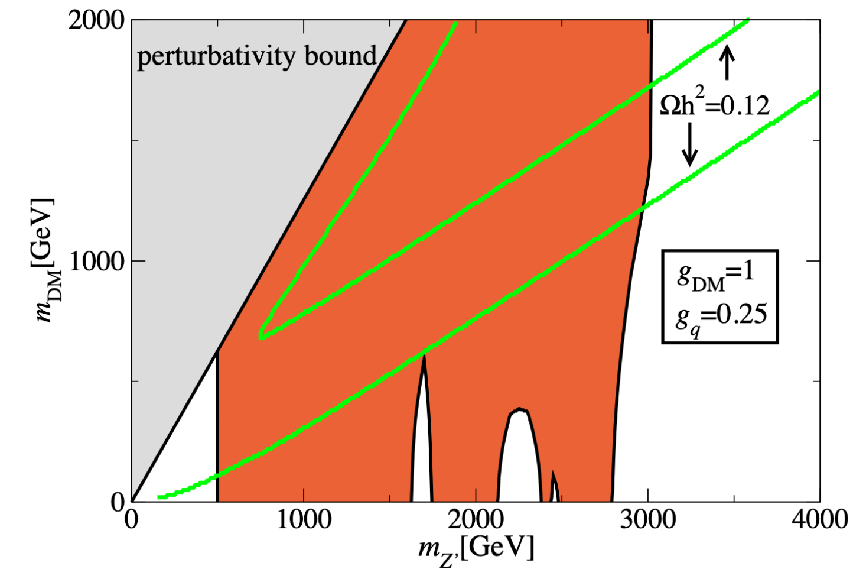
\includegraphics[width=0.9\textwidth]{Figures/2/Zprime_constrants_dijet.pdf}
\caption{Dijet resonance. Figure from $\copyright$ \cite{Zprime_portal_dijet}.}
\label{fig:Zprime_constraints_dijet}
\end{subfigure}
\begin{subfigure}[t]{0.54\textwidth}
	\centering
	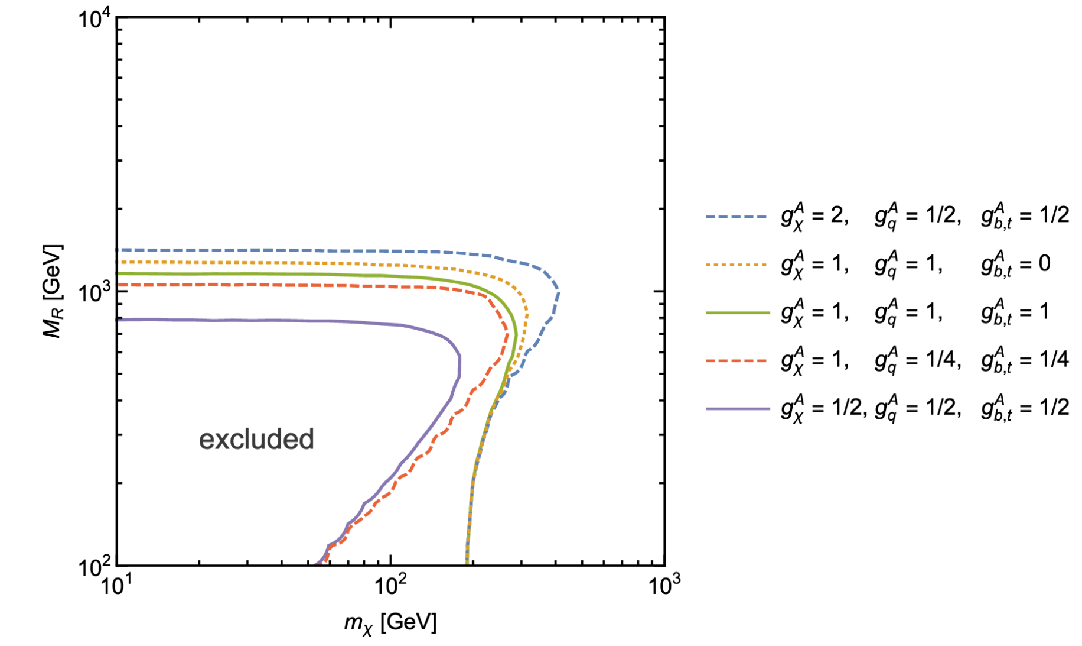
\includegraphics[width=0.99\textwidth]{Figures/2/Zprime_constrants_monojet.pdf}
\caption{Mono-jet. Figure from $\copyright$ \cite{Zprime_portal_monojet_dijet}.}
\label{fig:Zprime_constraints_monojet}
\end{subfigure}
	\caption{Constraints on the masses of the \Zprime vector boson mediator (labelled \mZp in \ref{fig:Zprime_constraints_dijet} and \(M_R\) in \ref{fig:Zprime_constraints_monojet}) and DM (labelled \(m_\text{DM}\) in \ref{fig:Zprime_constraints_dijet} and \(\mchi\) in \ref{fig:Zprime_constraints_monojet}) from combined ATLAS and CMS dijet searches \cite{Zprime_portal_monojet_dijet} (left) and mono-jet searches \cite{Zprime_portal_monojet_dijet} (right). The results are shown for typical coupling choices of the \Zprime to DM (\(g_\text{DM}\) in \ref{fig:Zprime_constraints_dijet} and \(g^A_\chi\) in \ref{fig:Zprime_constraints_monojet}), and of the \Zprime to quarks (\(g_q\) in \ref{fig:Zprime_constraints_dijet} and \(g^A_q\) or  \(g^A_{b,t}\) in \ref{fig:Zprime_constraints_monojet}, where \(g^A_{b,t}\) specifies the coupling to heavy quarks, which may be 0 for models which prohibit heavy quark couplings). Green lines in \ref{fig:Zprime_constraints_dijet} contain the region of \(\mZp, ~\mchi\) which reproduces the observed relic density of DM in the Universe. In the grey region perturbative unitarity \cite{Zprime_portal_monojet_dijet} is violated.}
	\label{fig:Feynman_Zprime}
\end{figure}

\subsection{Implications of a Dark Higgs Portal}

The implications of introducing a new portal interaction mediated by a spin 0 boson (the DH) - which couples to the SM via a mixing with the SM Higgs boson - to the generic \Zprime mediator portal discussed above are studied in detail by Duerr et al. in Ref. \cite{Duerr_2016}. In this study, it is found that within various regimes of the coupling strengths and masses of the hypothetical particles - the \Zprime, DH and DM - in this two-mediator model (2MDM), it is possible to relax or evade some of the constraints described above on the generic \Zprime mediator model from the combination of experimental results and the observed relic DM density in the Universe. As a result, in addition to providing a mechanism by which particles may acquire mass in the dark sector, the DH also introduces new parameter space to the model that is not yet excluded by existing constraints. In particular, for \(\ms < 2\mchi\) and provided there are no other lighter particles in the dark sector, the only available decay route for the \(s\) is to SM particles via mixing with the SM Higgs, regardless of the mixing strength. In this case, the DM relic abundance is predominately set by the process \(\chi\chi\rightarrow ss\) followed by decays of \(s\) into SM particles, which allows for a significant relaxation of relic density constraints. 

For various choices of \mchi, the study by Duerr et al. \cite{Duerr_2016} performs global scans over all possible choices of the coupling strengths (presented in Section \ref{sec:DH_model_description} below) that are in the 2MDM model, in the (\ms, \mZp) plane, as shown in Figure \ref{fig:Duerr_general_constraints}. Particularly for \(\mchi\geq200 ~\GeV\), it is found that all existing constraints can be evaded for a large region of \ms and \mZp (up to \(\sim1000~\GeV\) in \ms and up to \(\sim2500~\GeV\) in \mZp).

\begin{figure}[hp]
	\centering
	\centering
	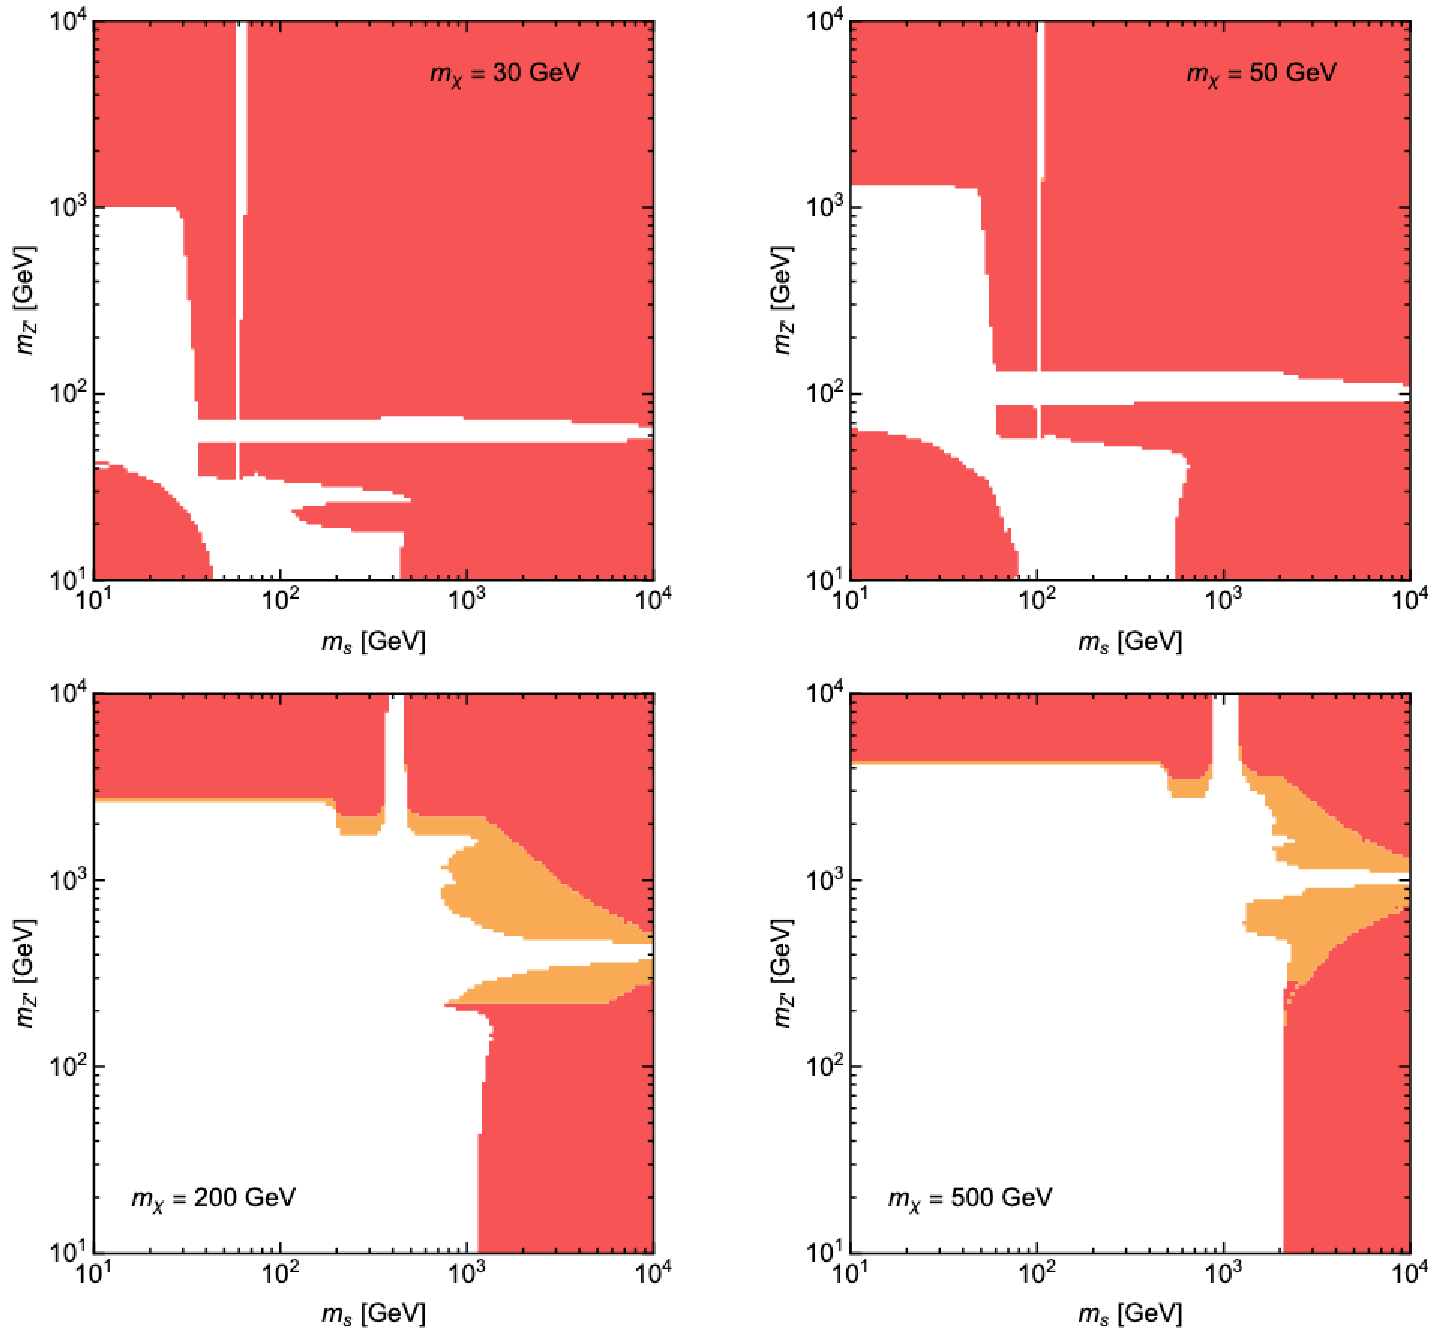
\includegraphics[width=0.8\textwidth]{Figures/2/Duerr_general_constraints.pdf}
	\caption{Global scans of the 2MDM model, with \Zprime and DH as portal mediators, performed by Duerr et al in Ref. \cite{Duerr_2016}. The red shaded region is excluded for all possible
combinations of couplings, while in the white region all constraints can be evaded. In the orange shaded region it is not possible to exclude large values of \(g_q\) , corresponding to \(\Gamma_\Zprime / \mZp > 0.3\). Figure from $\copyright$ \cite{Duerr_2016}.}
	\label{fig:Duerr_general_constraints}
\end{figure}

\section{Model Description}
\label{sec:DH_model_description}

The DH model, presented in Refs. \cite{Duerr_2016} and \cite{Duerr2017}, belongs to a wider class of simplified dark sector models which hypothesize that DM interacts with particles of the SM via the exchange of one or more new mediators, which act as so-called ``portals" between the SM and the dark sector. Candidate portals are broadly categorized according to the portal mediator into vector- \cite{vector_mediator_2012,vector_mediator_2020}, neutrino- \cite{neutrino_mediator_2019}, Higgs- \cite{higgs_mediator_2020} and axion-mediated \cite{axion_mediator_2009} portals. In this model, DM is assumed to be a Majorana fermion, which means that - like the photon, for example - it is its own antiparticle, and interacts with the SM via both vector-mediated and Higgs-mediated portals. 

A new gauge group called the U(1)' with an associated vector gauge boson, referred to as the \Zprime, is introduced as an extension of the SM gauge group presented in Chapter \ref{chapter:introduction}. Both the DM and and the \Zprime are assumed to obtain their mass from a new Higgs field with vaccum expectation value \(w\), which gives rise to a new physical Higgs boson, the DH boson \(s\). The DM acquires an axial coupling to the \Zprime, such that all three dark sector particles interact with one another. 

The interactions of the U(1)' gauge group within the dark sector are expressed by the interaction Lagrangian (of which more details can be found in Appendix A of Ref. \cite{Duerr_2016}):

\begin{equation}
\label{eq:DH_Lagrangian}
    \mathcal{L}_{U(1)'} = - \frac{1}{2} \gchi {\Zprime}^{\mu} \bar{\chi} \gamma^{5} \gamma_{\mu} \chi - \gchi \frac{\mchi}{\mZp} s \bar{\chi} \chi + 2 \gchi {\Zprime}^{\mu} {\Zprime}_{\mu} (\gchi s^2 + \mZp s)
\end{equation}

\noindent Considering each term in \(\mathcal{L}_{\chi}\) individually: 

\begin{equation}
\mathcal{L}_{\chi, \Zprime} = - \frac{1}{2} \gchi {\Zprime}^{\mu} \overline{\chi} \gamma^{5} \gamma_{\mu} \chi
\end{equation}

\noindent describes the axial coupling between the DM \(\chi\) and the \Zprime, with coupling strength \(g_\chi\). 

\begin{equation}
\label{eq:Lagrangian_chi_s}
\mathcal{L}_{\chi, \text{DH}} =- \gchi \frac{\mchi}{\mZp} s \bar{\chi} \chi = - \frac{y_\chi}{2\sqrt{2}} s \bar{\chi} \chi
\end{equation}

\noindent describes the coupling between the DM \(\chi\) and the Dark Higgs field, where the associated coupling strength \(y_\chi\) on the right-hand side of Eq. \ref{eq:Lagrangian_chi_s} has the following dependence on the masses and coupling strength of the DM and the \Zprime: \(y_\chi = 2\sqrt{2}g_\chi\frac{\mchi}{\mZp}\).

\begin{equation}
\mathcal{L}_{\Zprime, \text{DH}} = 2 \gchi {\Zprime}^{\mu} {\Zprime}_{\mu} (\gchi s^2 + \mZp s)
\end{equation}

\noindent describes the interaction between the \Zprime and the Dark Higgs field.

Motivated by models of gauged baryon number \cite{baryon_number,Duerr_2016,Duerr2017}, the SM quarks are charged under the U(1)' gauge group, and as a result interact with the \Zprime vector boson via vector coupling described by the following interaction Lagrangian:

\begin{equation}
\label{eq:quark_Zprime_coupling}
\mathcal{L}_{q, \Zprime} = -\gchi{\Zprime}^\mu\bar{q}\gamma_\mu q
\end{equation}

\noindent thus opening up a mechanism for vector-mediated portal interactions between the SM and the dark sector. 

 The most general Lagrangian describing the scalar Higgs \(h\) and Dark Higgs \(s\) is given by \cite{DH_SMHiggs_mixing_2016}:
 
 \begin{equation}
 \label{eq:scalar_lagrangian}
 \mathcal{L}_\mathcal{\text{scalar}} = -\lambda_h \Big(H^\dagger H - \frac{v^2}{2}\Big) - \lambda_s \Big(S^\dagger S - \frac{w^2}{2}\Big) - \lambda_{hs} \Big(H^\dagger H - \frac{v^2}{2}\Big) \Big(S^\dagger S - \frac{w^2}{2}\Big)
 \end{equation}
 
\noindent where \(H=\frac{1}{\sqrt{2}}(0, v+h)\) represents the SM Higgs field with vacuum expectation value \(h\), and \(S=\frac{1}{\sqrt{2}}(s+w)\) represents the Dark Higgs field. The third term with coupling \(\lambda_{hs}\) mixes the visible and dark sectors, such that the physical mass eigenstates \(h'\) and \(s'\) will be a superposition of the scalars \(h\) and \(s\):

\begin{equation}
\label{eq:higgs_mass_eigenstates}
\begin{pmatrix}
h' \\ s'
\end{pmatrix} = 
\begin{pmatrix}
\cos\theta & \sin\theta \\
\sin\theta & \cos\theta 
\end{pmatrix}
\begin{pmatrix}
h \\ s
\end{pmatrix}
\end{equation}

\noindent where the ``mixing angle" \(\theta\) is related to SM and Dark Higgs field couplings \(\lambda_h\) and \(\lambda_s\) and the vacuum expectation values \(v\) and \(w\) by:

\begin{equation}
\label{eq:higgs_mixing_angle}
\tan2\theta = \frac{\lambda_{hs}vw}{\lambda_hv^2 ? \lambda_sw^2}
\end{equation}

If the mixing (\(\sin\theta > 0\)) between the physical SM and Dark Higgs bosons is nonzero, the possibility 

%\begin{equation}
%\label{eq:}
%\end{equation}

\begin{itemize} 
\item Emphasize that $m_\chi>\frac{1}{2}\ms$ required to obtain signature in detector (otherwise $s\rightarrow\chi\chi$ decay would dominate).
\end{itemize}

\section{Search for the Dark Higgs Model at the LHC}

\begin{itemize}
\item Discussion of the model's signature in the ATLAS detector (boosted SM pair recoiling against \met), and why the boosted topology is unique compared with generic mono-X searches in which the `X' is produced via ISR.
\item Discussion of available search channels - mono-s(bb), mono-s(WW), mono-s(ZZ), mono-s(hh).
\begin{itemize}
\item Overview of existing searches for the Dark Higgs model - re-interpreted mono-h(bb), hadronic mono-s(WW). Could also mention ongoing dedicated mono-s(bb) search.
\item Identify the \ms regime in which the $s\rightarrow WW$ decay mode dominates in sensitivity.
\end{itemize}
\end{itemize}